In this section the operational items are sized. This can be summarised as the mass needed by the astronauts to live under reasonably comfortable conditions in the crew module during the mission. For this purpose the paper by Tito et al has been used \cite{Tito2013}. In this paper the operational items are called \acrfull{eclss}. First the method for estimation is described with its assumptions. Followed by the results of the estimation.

\paragraph{Estimation method}
The mass of the \gls{eclss} is primarily driven by the crew size and mission length. The \gls{eclss} is divided into subsystems: Air Management, Thermal and Humidity Management, Water Management, Waste Management, Human Accommodation, Food Preparation and Storage. Each of these subsystems can be subdivided into components. Examples of these are a water heater or packed food in the Food Preparation and Storage. It is evident that some components scale with the keydrivers and others do not. For example, adding a crew member does not necessitate an extra water heater, but it does require extra packed food. 


Taking this into account the mass has been divided into two components. A basic system mass which scales with crew size and the consumable mass that scales with crew size and mission length. Examples of components that belong to the basic system mass are oxygen scrubbers (not including oxygen), atmospheric control systems and food preparation systems. Examples of components that belong to consumable mass are oxygen, food, water and personal provisions. The used reference by Tito et al incorporates the mass for the \gls{tcs}. It is assumed that this \gls{tcs}-mass only provides the thermal control for the operational items. The \gls{tcs} for other subsystems is discussed in Section \ref{subsec:crewthermalcontrol}.

\paragraph{Results}
By using the method described in the previous paragraph the results of Table \ref{tab:operationalest} were obtained.
\begin{table}[h]
	\centering
	\caption{Obtained masses and volumes of basic system \& consumable items}
	\begin{tabular}{|p{1.9cm}|p{2.7cm}|p{2.7cm}|p{3.5cm}|p{3.6cm}|}
		\hline
		\textbf{Crew members} & \textbf{Basic system mass $[kg]$} & \textbf{Basic system volume $[m^{3}]$} & \textbf{Consumables mass per day $[kg]$} & \textbf{Consumables volume per day $[m^{3}]$} \\ \hline \hline
		1 & 1,800 & 4.88 & 3.2 & 0.018 \\
		2 & 2,500 & 6.78 & 6.4 & 0.036 \\
		3 & 3,200 & 8.68 & 9.6 & 0.054 \\
		\hline
	\end{tabular}
	\label{tab:operationalest}
\end{table}
It can be seen from Table \ref{tab:operationalest} that both the basic system and consumables mass scale with the number of crew members. By using linear extrapolation the mass and volume associated with crew members higher than three can be determined. These are shown in Table \ref{tab:crewmemberops} for a mission time of $100$ days, which incorporates the transfer from Earth to Mars and the maximum deceleration time. Herein the \gls{tcs}-mass for the operational items comes down to 480 $[kg]$.\\

\begin{table}[h!]
	\caption{Total mass and volume associated with operational items for varying crew numbers}
	\begin{tabular}{|c|c|c|}
		\hline
		\textbf{Crew members} & \textbf{Operational items mass $[kg]$} & \textbf{Operational items volume $[m^{3}]$}\\ \hline \hline
		1 & 2,120 & 6.69\\
		2 & 3,140 & 10.40\\
		3 & 4,160 & 14.11\\
		4 & 5,180 & 17.82\\
		5 & 6,200 & 21.53\\
		6 & 7,220 & 25.24\\ \hline
	\end{tabular}
	\label{tab:crewmemberops}
\end{table}
Furthermore Rudisill et al mention the spacecraft volume required for crew operations per crew member \cite{Rudisill2008}. This volume can take on three different values depending on the mission length. The resultant habitable volumes are shown in figure \ref{fig:crewvolume}.
\begin{figure}[h]
	\centering
	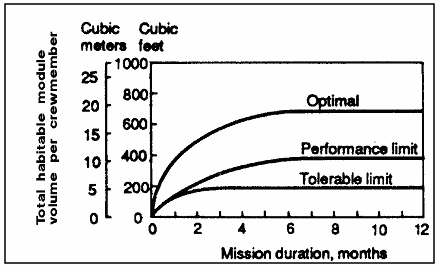
\includegraphics[scale=1.0]{./Figure/CrewModule/Crewvolume}
	\caption{Habitable volume per crew member as a function of mission duration \cite{Rudisill2008}}
	\label{fig:crewvolume}
\end{figure}
In the remainder of this report the crew habitable volume will be sized to the 'performance limit' indicated in figure \ref{fig:crewvolume}.
